\subsection{Automatic differentiation}
Automatic differentiation (\textit{AD}) has a long and rich history, where its driving motivation is to efficiently calculate the derivatives of functions in a manner that is both correct and fast\cite{Baydin2015AutomaticDI}.
There are several different methods of implementing AD algorithms, such as source-code transformations or operator overloading.
These algorithms usually transform any program which implements some function to one that calculates its derivative.

There are two main variants of AD, namely forward-mode and reverse-mode AD.
In forward-mode AD, we annotate every term in the function trace with their corresponding derivative.
These are also known as, respectively, the primal and tangent traces.
So calculating the partial derivatives of sub-terms is structural with respect to normal calculations.

This approach to forward-mode AD can be explained by what is mathematically known as dual numbers, as these are, in essence, what we are calculating\cite{Baydin2015AutomaticDI}. Dual numbers are numbers in the form of
$$
  x + x' \epsilon
$$
where $x, x' \in \denR$ and $\epsilon$ is a nilpotent number, such that $\epsilon^2 = 0$ and $\epsilon \neq 0$.
Notably, both primal and tangent values are tracked in this representation, namely the tangent value is equal to the coefficient of $\epsilon$.
As an example, we can see that this is true for both addition and multiplication:
\begin{align*}
  (x + x' \epsilon) + (y + y' \epsilon) &= (x + y) + (x' + y')\epsilon \\
  (x + x' \epsilon)(y + y' \epsilon) &= (xy) + (xy' + yx')\epsilon
\end{align*}
Using the following scheme for function application:
\begin{align*}
  f(x + x' \epsilon) &= f(x) + f'(x)x'\epsilon
\end{align*}
We can also see that it follows the chain rule for function composition.
\begin{align*}
  f(g(x + x' \epsilon)) &= f(g(x) + g'(x)x'\epsilon)) \\
    &= f(g(x)) + f'(g(x))g'(x)x'\epsilon
\end{align*}
Using this, we can essentially calculate the derivative of any differentiable function by interpreting any non-dual number $x$ as its dual number counterpart. Respectively, we interpret constant values as $x + 0\epsilon$, while input variables we take the partial derivative of, are interpreted as $x + 1\epsilon$.

To give a more elaborate example of how forward-mode AD works graphically, take the function $f(x, y) = x^2 + (x - y)$ as an example.
The dependencies between the terms and operations of the function is visible in the computational graph in \cref{fig:func_trace}.
The corresponding traces are filled in \cref{table:func_trace} for the input values $x = 2, y = 1$.
We can calculate the partial derivative $\frac{\delta f}{\delta x}$ at this point by setting $x' = 1$ and $y' = 0$.
Note that the calculation of the traces is structural.
This means that when we calculate the primal value at a specific point, we can calculate the corresponding tangent value at that same point.

\begin{figure}
  \centering
  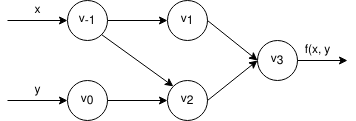
\includegraphics[scale=0.6]{./assets/function_trace.png}
  \caption{Computational graph of $f(x, y) = x^2 + (x - y)$}
  \label{fig:func_trace}
\end{figure}

\begin{table}
  \begin{center}
    \begin{tabular}{ l l l l l | l l l l l }
      \hline
      \multicolumn{5}{l}{Primal trace} & \multicolumn{5}{l}{Tangent trace} \\
      \hline
$v_{-1} $&$=$&$x$&$=$&$2$             &$v'_{-1}$&$=$&$x'$&$=$&$1$ \\
$v_0    $&$=$&$y$&$=$&$1$             &$v'_{0}$&$=$&$y'$&$=$&$0$ \\
      \hline
$v_1    $&$=$&$v_{-1}^2$&$=$&$4$      &$v'_{1}$&$=$&$2*v_{-1}$&$=$&$4$ \\
$v_2    $&$=$&$v_{-1} - v_{0}$&$=$&$1$&$v'_{2}$&$=$&$v'_{-1}-v'_{0}$&$=$&$1$ \\
$v_3    $&$=$&$v_1 + v_2$&$=$&$5$     &$v'_{3}$&$=$&$v'_1 + v'_2$&$=$&$5$ \\
      \hline
$f      $&$=$&$v_3$&$=$&$5$           &$f'$&$=$&$v'_3$&$=$&$5$ \\
      \hline
    \end{tabular}
  \end{center}
  \caption{Primal and tangent traces of $f(x, y) = x^2 + (x - y)$}
  \label{table:func_trace}
\end{table}

Reverse-mode automatic differentiation takes a drastically different approach.
It starts by annotating one of the possibly many output variables $\frac{\partial{y}}{\partial{y}} = 1$ and working in the reverse direction, annotating each intermediate variable $v_i$ with their adjoint
$$v'_i=\frac{\delta y_i}{\delta v_i}$$
To accomplish this, we require two separate passes.
Like the forward-mode variant, a primal trace is needed.
This first pass acts to determine the intermediate variables and their respective dependencies.
The second pass in the algorithm calculates the partial-derivatives by working backwards from the output using the adjoints, also called the adjoint trace.
The adjoints of multiple usages of the same variables, also called fan-out, are combined using addition in the adjoint trace.

The optimal choice between the automatic differentiation variants is heavily dependent on the function under consideration.
Preference is given for forward-mode AD when the number of output variables exceeds the number of input variables, as it has to be rerun for each partial derivative of the function.
On the other hand, reverse-mode AD scales with the number of output variables as it works backwards from each one.
In machine learning research, preference is given for reverse-mode AD, because the objective functions generally contain a small number of output variables.

While implementing forward-mode AD algorithms is very straightforward, reverse-mode AD is more problematic.
Correctly creating the reverse pass such that it handles both fan-out and zeroing in the reverse pass is difficult.
As such, many frameworks targeting non-theoretical applications such as deep learning focus on imperative languages, which eases the process due to the additional concept of state.

There are two main styles of implementing reverse-mode AD, namely define-then-run and define-by-run.
Define-then-run attempts to create the static computational graph during the compilation process that transforms the program to one that calculates the derivative of the function the program describes.
One significant benefit to this approach is the added opportunity to apply optimization steps in the compilation process.
This does currently, however, have the restriction that programs defined within these frameworks are limited in their usage of intricate control flow.

This restriction is lifted in the define-by-run style, which builds the computation graph during runtime.
As such, conditionals and loops can now be used freely in the framework.
On the other hand, as the computation graph is constructed during runtime, define-by-run frameworks can be slower due to the missing opportunities to apply optimizations.
Frameworks using this style are Chainer\fancyfootnote{https://chainer.org/} and PyTorch\fancyfootnote{https://pytorch.org/}
